\documentclass[main.tex]{subfiles} % Subfile-Class

%==============================================================================%
%                                   Subfile                                    %
%==============================================================================%

\begin{document}

\section{Risikomanagement}~\label{apx:risikoanalyse}

Das Risikomanagement wird nach der ALARP-Methode (\textit{engl. as low as
    reasonably possible}) durchgeführt. Dafür werden Risiken im ersten Schritt
identifiziert und anschliessend durch risikomindernde Massnahmen auf ein Niveau
reduziert, das ein angemessenes Mass an Sicherheit bietet. Die Bewertung
erfolgt im gesamten Team und basiert auf einer subjektiven Einschätzung zur
Erfüllung der Aufgabe. Ziel ist es, möglichst früh im Projektverlauf kritische
Punkte zu identifizieren und den Fokus auf diese zu legen. \

% -------------------------------------- Erläuterung Bewertung

\subsubsection*{Eintrittswahrscheinlichkeit (EW)}

Die Eintrittswahrscheinlichkeit ist ein Mass für die Wahrscheinlichkeit, mit
der ein Ereignis eintreten könnte.

\begin{table}[H] \begin{tabularx}{\textwidth}{|>{\centering\arraybackslash}p{1cm}|>{\raggedright\arraybackslash}X|>{\centering\arraybackslash}p{2cm}|}
        \hline
        \textbf{EW} & \textbf{Bezeichnung} & \textbf{\%} \\
        \hline
        6           & häufig               & $>90\%$     \\
        \hline
        5           & wahrscheinlich       & $>70\%$     \\
        \hline
        4           & gelegentlich         & $>50\%$     \\
        \hline
        3           & entfernt vorstellbar & $>30\%$     \\
        \hline
        2           & unwahrscheinlich     & $>15\%$     \\
        \hline
        1           & unvorstellbar        & $>5\%$      \\
        \hline
    \end{tabularx}
    \caption{Legende Eintrittswahrscheinlichkeit}~\label{tab
    } \end{table}

\subsubsection*{Schadensausmass (SA)}

Das Schadensausmass ist ein Mass dafür, wie fatal ein eintretendes Ereignis für
den Projekterfolg ist.

\begin{table}[H]
    \begin{tabularx}{\textwidth}{|>{\centering\arraybackslash}p{1cm}|>{\raggedright\arraybackslash}X|>{\raggedright\arraybackslash}X|}
        \hline
        \textbf{SA} & \textbf{Bezeichnung} & \textbf{Auswirkung}          \\
        \hline
        4           & katastrophal         & Wettbewerb abgebrochen       \\
        \hline
        3           & kritisch             & Gefährdung für Projekterfolg \\
        \hline
        2           & geringfügig          & Minderung des Projekterfolgs \\
        \hline
        1           & unwesentlich         & Störung des Projekterfolgs   \\
        \hline

    \end{tabularx}
    \caption{Legende Schadensausmass}~\label{tab:Legende_Schadensausmass}
\end{table}

\subsubsection*{Bereichsdefinition}

Die entsprechenden Risiken sind mit der folgenden Farbgebung codiert, um die
Notwendigkeit von Massnahmen zu kennzeichnen.

\begin{table}[H]
    \centering
    \begin{tabular}{|c|c|}
        \hline
        Farbcodierung         & Bedeutung             \\
        \hline
        \cellcolor{green!30}  & Akzeptabler Bereich   \\
        \hline
        \cellcolor{yellow!30} & ALARP-Bereich         \\
        \hline
        \cellcolor{red!30}    & Inakzeptabler Bereich \\
        \hline
    \end{tabular}
    \caption{Legende Bereichsdefinition}~\label{tab:Legende_Bereichsdefinition}
\end{table}

\newcounter{counter}
\setcounter{counter}{0}

\subsection*{Erkannte Risiken}

Im nachfolgenden Abschnitt sind die Risiken aufgeführt, die zum Semesterstart
festgestellt wurde. Auf Basis dieser Analyse ist der Fokus bei verschiedenen
Arbeiten besser aufgeteilt worden.

Die Risiken sind in die vier Bereiche Allgemeines, Maschinenbau, Elektrotechnik
und Informatik unterteilt. Ergänzend dazu wird aufgeführt, in welchem Sprint
das Risiko relevant wurde, wie die Eintrittswahrscheinlichkeit sowie das
Schadensausmass aussehen. Diese Risiken sind zum Start eines jeden Sprints neu
bewertet und bei der Aufgabenplanung mit einer höheren Priorität versehen.

\subsubsection* {Allgemeines}
\setcounter{counter}{0}
\begin{table}[H]
    \begin{tabularx}{\textwidth}{|>{\centering\arraybackslash}p{0.5cm}|>{\raggedright\arraybackslash}p{1.5cm}|>{\raggedright\arraybackslash}X|>{\centering\arraybackslash}p{0.75cm}|>{\centering\arraybackslash}p{0.75cm}|>{\raggedright\arraybackslash}X|}
        \hline
        \textbf{\#}                                                          & \textbf{Sprint} & \textbf{Risiko}                                       & \textbf{SA} & \textbf{EW} & \textbf{Auswirkungen}                                          \\

        \hline
        % ---------------------------------------------------------------------------------------------------------------------------------------------------------
        \rowcolor{yellow!30}
        \refstepcounter{counter}~\label{tabrow:risks_1_1} 1.\arabic{counter} & Alle            & Ausfall durch Krankheit oder Militär                  & 3           & 2           & Arbeiten verzögern sich.                                       \\
        \hline
        % ---------------------------------------------------------------------------------------------------------------------------------------------------------
        \rowcolor{green!30}
        \refstepcounter{counter}~\label{tabrow:risks_1_2} 1.\arabic{counter} & Alle            & Belastung durch Abgaben für andere Module nebst PREN2 & 2           & 2           & Arbeiten verzögern sich oder werden nicht sorgfältig erledigt. \\
        \hline
        % ---------------------------------------------------------------------------------------------------------------------------------------------------------
        \rowcolor{yellow!30}
        \refstepcounter{counter}~\label{tabrow:risks_1_3} 1.\arabic{counter} & Alle            & verpasste Sprintziele                                 & 3           & 2           & Demotivation \& Kürzungen bei zu erfüllenden Teilfunktionen.   \\
        \hline

    \end{tabularx}
    \caption{Erkannte Risiken aus dem allgemeinen Bereich}
\end{table}

\subsubsection *{Maschinenbau}
\setcounter{counter}{0}
\begin{table}[H]

    \begin{tabularx}{\textwidth}{|>{\centering\arraybackslash}p{0.5cm}|>{\raggedright\arraybackslash}p{1.5cm}|>{\raggedright\arraybackslash}X|>{\centering\arraybackslash}p{0.75cm}|>{\centering\arraybackslash}p{0.75cm}|>{\raggedright\arraybackslash}X|}
        \hline
        \textbf{\#}                                                          & \textbf{Sprint} & \textbf{Risiko}                                                    & \textbf{SA} & \textbf{EW} & \textbf{Auswirkungen}                                                                          \\

        \hline
        % ---------------------------------------------------------------------------------------------------------------------------------------------------------
        \rowcolor{green!30}
        \refstepcounter{counter} 2.\arabic{counter}~\label{tabrow:risks_2_1} & Prepare         & Fehldruck vom 3D Drucker                                           & 1           & 3           & Vorbereitungsphase verzögert sich                                                              \\
        \hline

        % ---------------------------------------------------------------------------------------------------------------------------------------------------------
        \rowcolor{green!30}
        \refstepcounter{counter} 2.\arabic{counter}~\label{tabrow:risks_2_2} & Prepare         & Beim Zusammenbau des Roboters bricht ein Teil                      & 1           & 3           & Vorbereitungsphase verzögert sich                                                              \\
        \hline
        % ---------------------------------------------------------------------------------------------------------------------------------------------------------
        \rowcolor{green!30}
        \refstepcounter{counter} 2.\arabic{counter}~\label{tabrow:risks_2_3} & Prepare         & Laufkugel bleibt hängen in Fuge                                    & 2           & 2           & Es muss ein neuer Adapter angefertigt werden für eine grössere Laufkugel.                      \\
        \hline
        % ---------------------------------------------------------------------------------------------------------------------------------------------------------
        \rowcolor{yellow!30}
        \refstepcounter{counter} 2.\arabic{counter}~\label{tabrow:risks_2_4} & 1               & Durchdrehen der Räder bei Beschleunigung                           & 2           & 4           & Fahrgeschwindigkeit muss reduziert werden. Hindernispositionierung nicht so genau wie geplant. \\
        \hline
        % ---------------------------------------------------------------------------------------------------------------------------------------------------------
        \rowcolor{yellow!30}
        \refstepcounter{counter} 2.\arabic{counter}~\label{tabrow:risks_2_5} & 1               & Kamerapositionierung nicht stabil genug für zuverlässige Aufnahmen & 3           & 1           & Anpassung der Kamera-Halterung notwendig.                                                      \\
        \hline
        % ---------------------------------------------------------------------------------------------------------------------------------------------------------
        \rowcolor{yellow!30}
        \refstepcounter{counter} 2.\arabic{counter}~\label{tabrow:risks_2_6} & 2               & Maximalgewicht wird nicht eingehalten                              & 2           & 4           & Chassiskonzept muss nochmals überarbeitet werden, um noch mehr Gewicht einzusparen.            \\
        \hline
        % ---------------------------------------------------------------------------------------------------------------------------------------------------------
        \rowcolor{green!30}
        \refstepcounter{counter} 2.\arabic{counter}~\label{tabrow:risks_2_7} & Alle            & Bauteildimensionierung zu schwach - es nehmen Bauteile Schaden     & 1           & 3           & Es müssen Bauteile neu gefertigt werden.                                                       \\
        \hline

    \end{tabularx}
    \caption{Erkannte Risiken aus dem Bereich der Mechanik}
\end{table}

\subsubsection* {Elektrotechnik}
\setcounter{counter}{0}
\begin{table}[H]
    \begin{tabularx}{\textwidth}{|>{\centering\arraybackslash}p{0.5cm}|>{\raggedright\arraybackslash}p{1.5cm}|>{\raggedright\arraybackslash}X|>{\centering\arraybackslash}p{0.75cm}|>{\centering\arraybackslash}p{0.75cm}|>{\raggedright\arraybackslash}X|}
        \hline
        \textbf{\#}                                                          & \textbf{Sprint} & \textbf{Risiko}                                                         & \textbf{SA} & \textbf{EW} & \textbf{Auswirkungen}                                                                                         \\

        \hline
        % ---------------------------------------------------------------------------------------------------------------------------------------------------------
        \rowcolor{green!30}
        \refstepcounter{counter}~\label{tabrow:risks_3_1} 3.\arabic{counter} & Prepare         & Beim Zusammenlöten der Prints kam es zu Fehlern                         & 1           & 3           & Vorbereitungsphase verzögert sich.                                                                            \\
        \hline
        % ---------------------------------------------------------------------------------------------------------------------------------------------------------
        \rowcolor{yellow!30}
        \refstepcounter{counter}~\label{tabrow:risks_3_2} 3.\arabic{counter} & 2               & Powerbudget ist nicht ausreichend                                       & 3           & 3           & Es müssen Einsparungen bei der Leistung der Motoren getroffen werden                                          \\
        \hline
        % ---------------------------------------------------------------------------------------------------------------------------------------------------------
        \rowcolor{green!30}
        \refstepcounter{counter}~\label{tabrow:risks_3_3} 3.\arabic{counter} & 1               & Bei Printplattenentwicklung kam es zu Fehlern                           & 3           & 3           & Das Konzept muss umgestellt werden, Aufgaben z.B. von anderen PCB's übernommen.                               \\
        \hline
        % ---------------------------------------------------------------------------------------------------------------------------------------------------------
        \rowcolor{green!30}
        \refstepcounter{counter}~\label{tabrow:risks_3_4} 3.\arabic{counter} & 1               & RS422 Schnittstelle und das Busprotokoll funktioniert nicht zuverlässig & 1           & 2           & Es sind Steckplätze zum Überbrücken dieser Schnittstelle vorgesehen, darauf muss dann zurückgegriffen werden. \\
        \hline
        % ---------------------------------------------------------------------------------------------------------------------------------------------------------
        \rowcolor{red!30}
        \refstepcounter{counter}~\label{tabrow:risks_3_5} 3.\arabic{counter} & Alle            & Elektronische Bauteile nehmen währrend des Erprobens Schaden            & 3           & 4           & Das Fahrzeug kann nicht weiter betrieben werden. Gegebenenfalls ist mit langen Wartezeiten zu rechnen.        \\
        \hline

    \end{tabularx}
    \caption{Erkannte Risiken aus dem Bereich der Elektrotechnik}
\end{table}

\subsubsection* {Informatik}
\setcounter{counter}{0}
\begin{table}[H]
    \begin{tabularx}{\textwidth}{|>{\centering\arraybackslash}p{0.5cm}|>{\raggedright\arraybackslash}p{1.5cm}|>{\raggedright\arraybackslash}X|>{\centering\arraybackslash}p{0.75cm}|>{\centering\arraybackslash}p{0.75cm}|>{\raggedright\arraybackslash}X|}
        \hline
        \textbf{\#}                                                          & \textbf{Sprint} & \textbf{Risiko}                                                  & \textbf{SA} & \textbf{EW} & \textbf{Auswirkungen}                                                                                                                            \\
        \hline
        % ---------------------------------------------------------------------------------------------------------------------------------------------------------
        \rowcolor{green!30}
        \refstepcounter{counter}~\label{tabrow:risks_4_1} 4.\arabic{counter} & Prepare         & Kommunikation zwischen Controllern funktioniert nicht            & 3           & 1           & Vorbereitungsphase verzögert sich, ggf. muss alternative Kommunikation implementiert werden.                                                     \\
        \hline
        % ---------------------------------------------------------------------------------------------------------------------------------------------------------
        \rowcolor{red!30}
        \refstepcounter{counter}~\label{tabrow:risks_4_2} 4.\arabic{counter} & 1               & Bildverarbeitung (Interpretation) funktioniert nicht zuverlässig & 4           & 3           & Algorithmus muss angepasst werden, was zu Verzögerungen führen kann.                                                                             \\
        \hline
        % ---------------------------------------------------------------------------------------------------------------------------------------------------------
        \rowcolor{green!30}
        \refstepcounter{counter}~\label{tabrow:risks_4_3} 4.\arabic{counter} & 1               & Prozessorleistung für die Bildverarbeitung ist zu gering         & 3           & 2           & Leistungsoptimierung (andere Programmiersprache) oder Hardware-Upgrade erforderlich, Zeitplan kann sich verzögern.                               \\
        \hline
        % ---------------------------------------------------------------------------------------------------------------------------------------------------------
        \rowcolor{yellow!30}
        \refstepcounter{counter}~\label{tabrow:risks_4_4} 4.\arabic{counter} & 2               & Mit LIDAR kann Pylon nicht genau lokalisiert werden              & 4           & 2           & Es muss nach einer anderen Möglichkeit gesucht werden, die Pylonen zu lokalisieren, oder die Positionierung der Sensorposition optimiert werden. \\
        \hline
    \end{tabularx}
    \caption{Erkannte Risiken aus dem Bereich der Informatik}
\end{table}

% ---------------------------------------- MASSNAHMEN ----------------------------------------------------------
\subsection*{Massnahmen für Risiken}

Die nachfolgenden Tabellen zeigen auf, welche Massnahmen zu den kritischen
Risiken (Farbmarkierung mindestens gelb) getroffen sind, um diese
einzuschränken. Dazu ist immer noch jeweils schematisch in einer Abbildung
gezeigt, wie die entsprechende Massnahme auf das Risiko wirkt.

\begin{description}
    \item[Allgemein] Tabelle~\ref{tab:Erfasste_Massnahmen_allg} \&
        Abbildung~\ref{fig:Diagramm_Risiko_allg}
    \item[Mechanik] Tabelle~\ref{tab:Erfasste_Massnahmen_mech} \&
        Abbildung~\ref{fig:Diagramm_Risiko_mech}
    \item[Elektrotechnik] Tabelle~\ref{tab:Erfasste_Massnahmen_elektro} \&
        Abbildung~\ref{fig:Diagramm_Risiko_elektro}
    \item[Informatik] Tabelle~\ref{tab:Erfasste_Massnahmen_info} \&
        Abbildung~\ref{fig:Diagramm_Risiko_info}
\end{description}

Manche Risiken können leider nicht weiter reduziert werden und müssen so wie
sie sind akzeptiert werden. Dazu zählt zum Beispiel der Personalausfall durch
Krankheit.

% ========= ALLGEMEIN

\subsubsection*{Allgemein}

\begin{table}[H]
    \begin{tabularx}{\textwidth}{|>{\centering\arraybackslash}p{2cm}|>{\raggedright\arraybackslash}X|>{\centering\arraybackslash}p{0.75cm}|}
        \hline
        \textbf{Risiko \#}        & \textbf{Massnahme}
                                  & \textbf{Neu EW}                                                                                                                                                                                                                                                                       \\
        \hline
        \rowcolor{yellow!30}
        1.~\ref{tabrow:risks_1_1} & Auf den Ausfall durch Krankheit hat man wenig Einfluss. Wichtig ist, dass alle Teammitglieder über die Tätigkeiten des jeweils anderen Informiert sind - damit das Team bei Ausfällen nicht blockiert wird. Die Auftretenswahrscheinlichkeit wird dadurch allerdings nicht reduziert.
                                  & 2                                                                                                                                                                                                                                                                                     \\
        \hline
        % ---------------------------------------------------------------------------------------------------------------------------------------------------------
        \rowcolor{green!30}
        1.~\ref{tabrow:risks_1_3} & Der Projektstand muss regelmässig abegprüft werden und Prioritäten entsprechend gesetzt. Alle Teammitglieder sind sich einig, dass keine Scham angebracht ist, den anderen zu kommunizieren, dass ein Ziel nicht erreicht werden kann.
                                  & 1                                                                                                                                                                                                                                                                                     \\
        \hline
    \end{tabularx}
    \caption{Erfasste Massnahmen für allgemein betreffende Risiken}~\label{tab:Erfasste_Massnahmen_allg}
\end{table}

\begin{figure}[H]
    \centering
    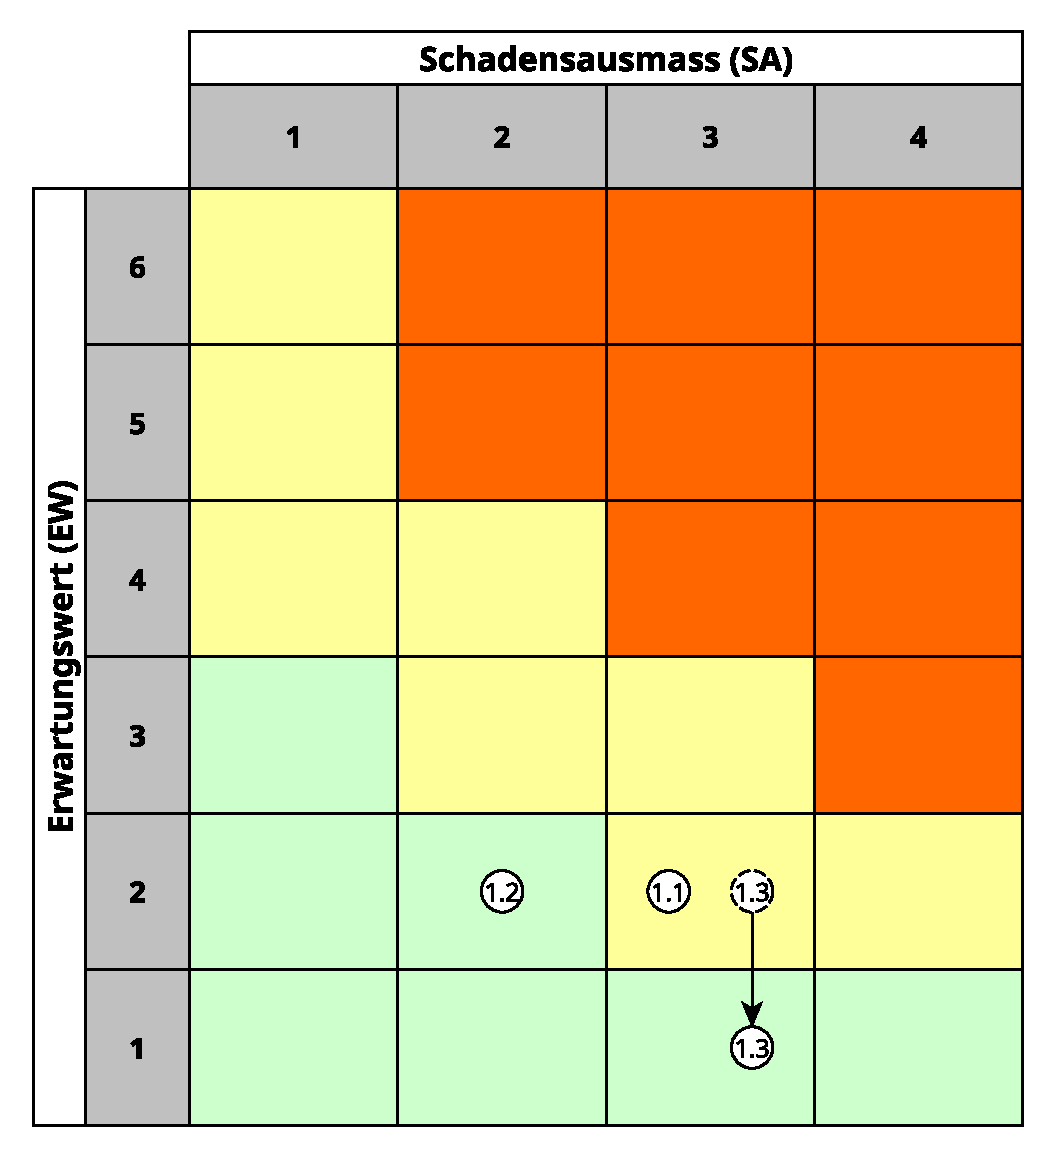
\includegraphics[width=0.75\textwidth]{./fig_Projektmanagement/Diagramm_Risiko_allg.pdf}
    \caption{Grafische Darstellung der Risikoanalyse Allgemein}~\label{fig:Diagramm_Risiko_allg}
\end{figure}

% ========= MECHANIK

\subsubsection*{Mechanik}

\begin{table}[H]
    \begin{tabularx}{\textwidth}{|>{\centering\arraybackslash}p{2cm}|>{\raggedright\arraybackslash}X|>{\centering\arraybackslash}p{0.75cm}|}
        \hline
        \textbf{Risiko \#}        & \textbf{Massnahme}
                                  & \textbf{Neu EW}                                                                                                                                                                                                                                                                               \\
        \hline
        \rowcolor{yellow!30}
        2.~\ref{tabrow:risks_2_4} & Die Traktion der Räder muss frühzeitig geprüft werden. Allenfalls muss die Maximale Beschleunigung, mit welcher die Räder beanschlagt werden, reduziert werden. Ausgeschaltet ist das Risiko allerdings nicht, da Umwelteinflüsse, wie ein staubiger Boden, nicht ausgeschlossen werden kann.
                                  & 3                                                                                                                                                                                                                                                                                             \\
        \hline
        % ---------------------------------------------------------------------------------------------------------------------------------------------------------
        \rowcolor{green!30}
        2.~\ref{tabrow:risks_2_5} & Der Turm, der die Kamera hält, wird mit besonderem Augenmerk auf die Steifigkeit designt. Darüber hinaus wird bei den ersten Probefaherten in Sprint 1 bereits mit Live-Material geprüft, wie stark das Zittern bemerkbar ist.
                                  & 2                                                                                                                                                                                                                                                                                             \\
        \hline
        % ---------------------------------------------------------------------------------------------------------------------------------------------------------
        \rowcolor{green!30}
        2.~\ref{tabrow:risks_2_6} & Dies wird einer der Haupt-Fokusse des Maschinenbau-Bereichs sein für das kommende Semester. Mit diesem erhöhten Zeitaufwand wird ein Chassis entstehen, welches besonders leicht ist.
                                  & 1                                                                                                                                                                                                                                                                                             \\
        \hline
        % ---------------------------------------------------------------------------------------------------------------------------------------------------------

        \hline
    \end{tabularx}
    \caption{Erfasste Massnahmen für den Mechanikbereich betreffende Risiken}~\label{tab:Erfasste_Massnahmen_mech}
\end{table}

\begin{figure}[H]
    \centering
    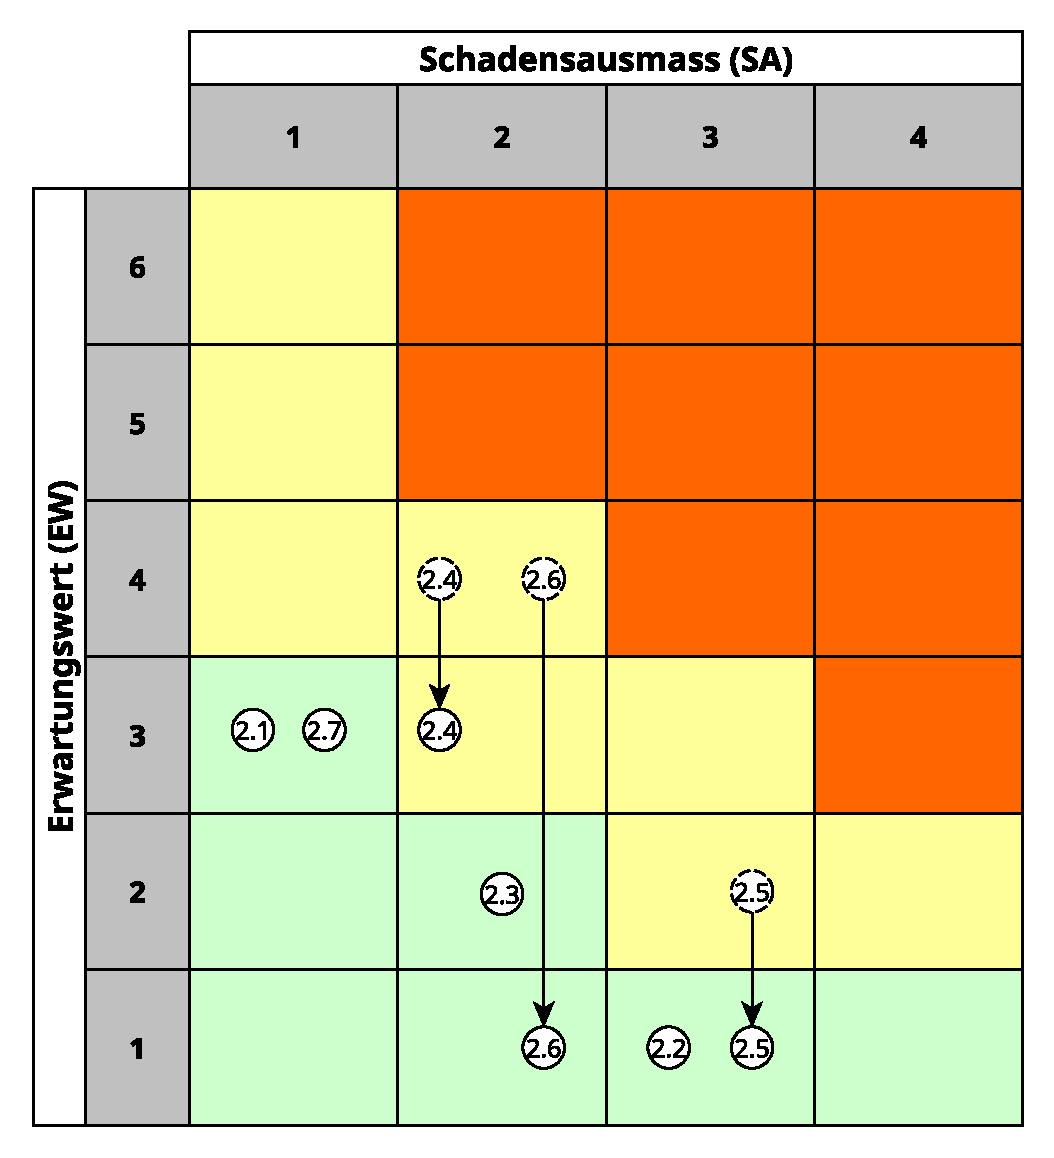
\includegraphics[width=0.75\textwidth]{./fig_Projektmanagement/Diagramm_Risiko_mechanik.pdf}
    \caption{Grafische Darstellung der Risikoanalyse Mechanik}~\label{fig:Diagramm_Risiko_mech}
\end{figure}

% ========= ELEKTROTECHNIK

\subsubsection*{Elektronik}

\begin{table}[H]
    \begin{tabularx}{\textwidth}{|>{\centering\arraybackslash}p{2cm}|>{\raggedright\arraybackslash}X|>{\centering\arraybackslash}p{0.75cm}|}
        \hline
        \textbf{Risiko \#}        & \textbf{Massnahme}
                                  & \textbf{Neu EW}                                                                                                                                                                                                                                                                                                                              \\
        \hline
        \rowcolor{yellow!30}
        3.~\ref{tabrow:risks_3_2} & Das Power-Budget muss frühzeitig getestet werden: Reicht die Akkulaufzeit? Erhalten die Motoren genügend Strom? Laufen die Controller stabil? All das muss früh getestet sein. Dieser punkt bleibt allerdings kritisch, da grosse Motoren verbaut sind und unsicher ist, ob gegebenenfalls auf einen Raspberry Pi 5 umgestiegen werden muss.
                                  & 2                                                                                                                                                                                                                                                                                                                                            \\
        \hline
        % ---------------------------------------------------------------------------------------------------------------------------------------------------------
        \rowcolor{green!30}
        3.~\ref{tabrow:risks_3_3} & Alle Printplatten müssen mit höchster Priorität zu beginn des Projekts zusammengebaut und inbetriebgenommen werden, damit frühzeitig noch alternativen wie neue PCB's oder etwa Teilfunktionen von anderen Leiterplatten übernommen werden können. Dadurch wird das Eintreten kritischer Situationen drastisch reduziert.
                                  & 1                                                                                                                                                                                                                                                                                                                                            \\
        \hline
        % ---------------------------------------------------------------------------------------------------------------------------------------------------------
        \rowcolor{yellow!30}
        3.~\ref{tabrow:risks_3_5} & Dass Bauteile beim Betrieb und bei Versuchen zu Schaden kommen lässt sich nur schwer ausschliessen. Es wird sichergestellt, dass kritische Bauteile wie Spannungsregler und Mikrokontroller als Ersatzteile vorliegen, dieser Punkt bleibt allerdings kritisch.
                                  & 2                                                                                                                                                                                                                                                                                                                                            \\
        \hline
    \end{tabularx}
    \caption{Erfasste Massnahmen für den Elektronikbereich betreffende Risiken}~\label{tab:Erfasste_Massnahmen_elektro}
\end{table}

\begin{figure}[H]
    \centering
    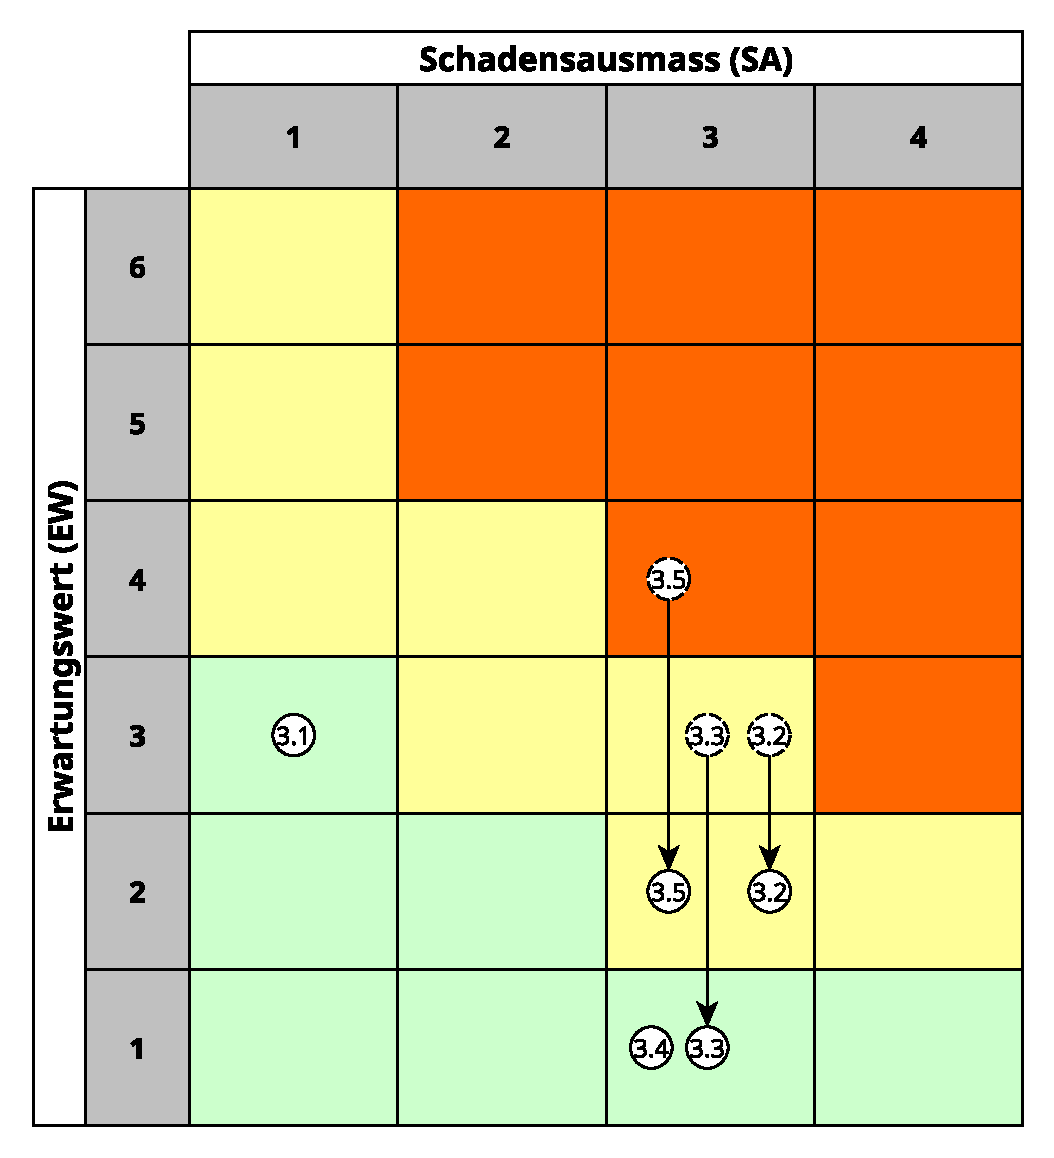
\includegraphics[width=0.75\textwidth]{./fig_Projektmanagement/Diagramm_Risiko_elektro.pdf}
    \caption{Grafische Darstellung der Risikoanalyse Elektrotechnik}~\label{fig:Diagramm_Risiko_elektro}
\end{figure}

% ========= INFORMATIK

\subsubsection*{Informatik}

\begin{table}[H]
    \begin{tabularx}{\textwidth}{|>{\centering\arraybackslash}p{2cm}|>{\raggedright\arraybackslash}X|>{\centering\arraybackslash}p{0.75cm}|}
        \hline
        \textbf{Risiko \#}        & \textbf{Massnahme}
                                  & \textbf{Neu EW}                                                                                                                                                                                                                                                                    \\
        \hline
        \rowcolor{yellow!30}
        4.~\ref{tabrow:risks_4_2} & Die Bild wird von Semesterbeginnn an mit besonderem Fokus bearbeitet. Es bleibt allerdings ein Risiko.
                                  & 2                                                                                                                                                                                                                                                                                  \\
        \hline
        % ---------------------------------------------------------------------------------------------------------------------------------------------------------
        \rowcolor{yellow!30}
        4.~\ref{tabrow:risks_4_4} & Ob Pylonen gut erkannt werden können, kann leider erst relativ spät im Semster geklärt werden. Vorgängige Tests bezüglich der Sensorgenauigkeit lassen allerdings darauf schliessen, dass die Eintretenswahrscheinlichkeit eher gering ist, deshalb wird dieses Risiko akzeptiert.
                                  & 2                                                                                                                                                                                                                                                                                  \\
        \hline
        % ---------------------------------------------------------------------------------------------------------------------------------------------------------
        \\
        \hline
    \end{tabularx}
    \caption{Erfasste Massnahmen für den Informatikbereich betreffende Risiken}~\label{tab:Erfasste_Massnahmen_info}
\end{table}

\begin{figure}[H]
    \centering
    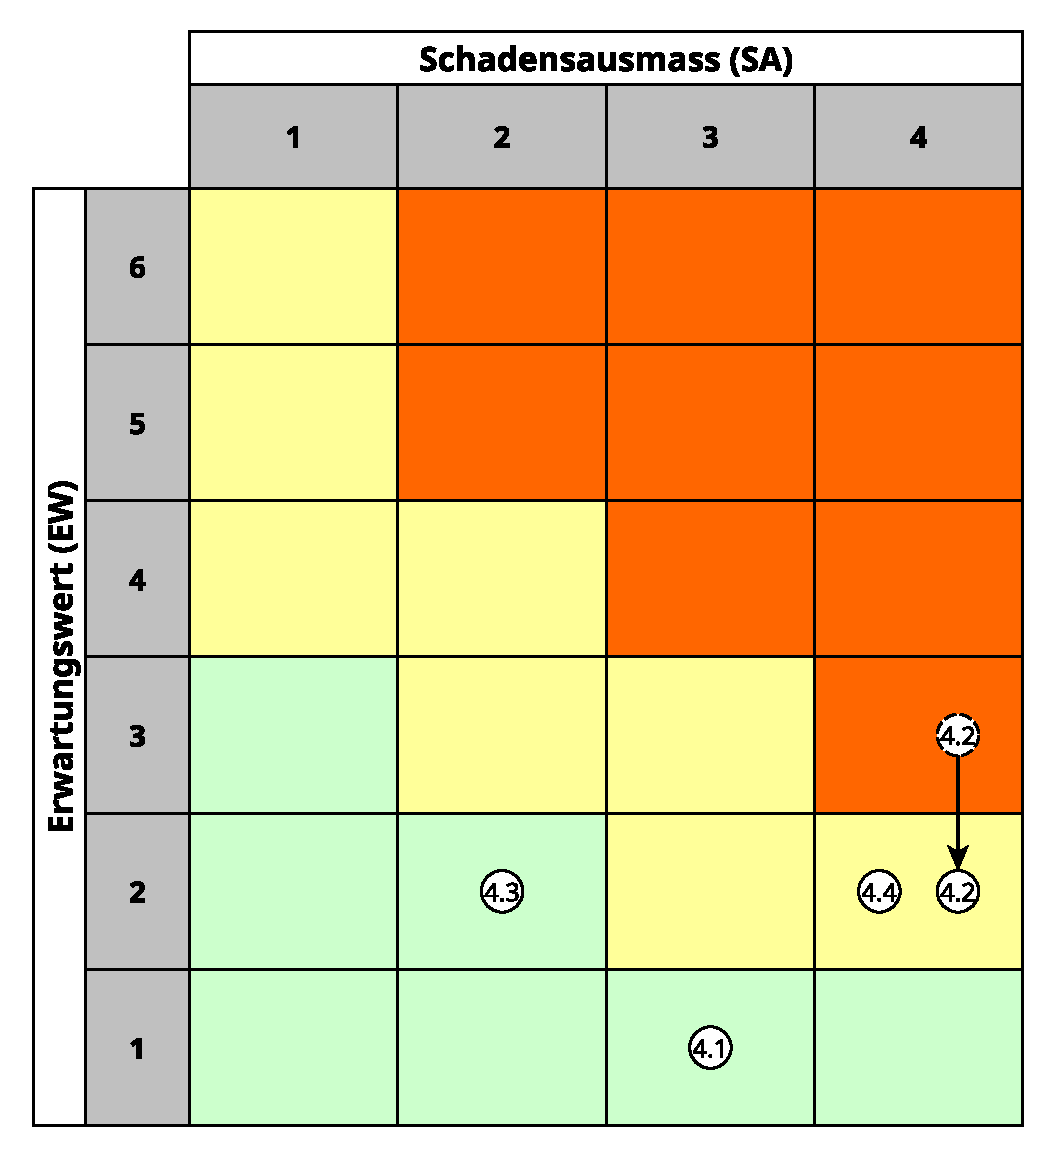
\includegraphics[width=0.75\textwidth]{./fig_Projektmanagement/Diagramm_Risiko_info.pdf}
    \caption{Grafische Darstellung der Risikoanalyse Informatik}~\label{fig:Diagramm_Risiko_info}
\end{figure}

\end{document}